\subsection{Modelo matemático do sistema de suspensão não linear para um quarto de veículo }
O modelo de um quarto de carro consiste em isolar uma quarta parte do veículo e estudar isoladamente o comportamento do sistema de suspensão para esta seção. Para veículos com peso igualmente distribuído, os resultados são muito próximos ao do modelo completo. Geralmente os modelos para um quarto de carro tem 2 graus de liberdade, sendo estes o deslocamento vertical da massa suspensa e da massa não suspensa, o que pode ser observado na figura \ref{fig:massa_mola_nao_linear_controlavel} a seguir. Este modelo é composto por uma massa suspensa que representa a carroceria do veículo e uma massa não suspensa que representa o conjunto eixo e roda. Estas massas são conectadas pela mola e pelo amortecedor. O contato do veículo com a pista de rolamento é realizado através do pneu. O sistema é exitado, ou perturbado, pelas irregularidades da pista.
\FloatBarrier
\begin{figure}[htbp]
    \begin{centering}
        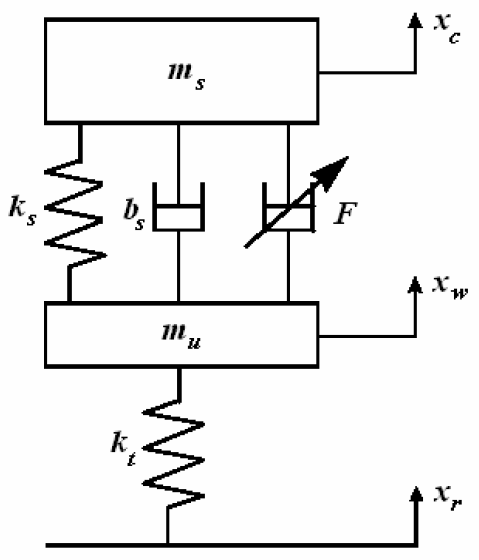
\includegraphics[width=8cm,height=6cm]{img/massa_mola_nao_linear_controlavel.png}
        \caption{Modelo de suspensão para um quarto de carro.} 
        \label{fig:massa_mola_nao_linear_controlavel}
    \end{centering}
\end{figure}
\FloatBarrier
Na figura \ref{fig:massa_mola_nao_linear_controlavel}, $m_s$ representa a massa suspensa que consiste em um quarto da massa total da carroceria do veículo em \emph{kg}, $m_u$ representa a massa não suspensa ou a massa do eixo e da roda em \emph{kg}, $b_s$ representa o coeficiente de amortecimento do amortecedor passivo em \emph{Ns/m}, $k_s$ representa o coeficiente de elasticidade do feixe de molas da suspensão, segundo a lei de Hooke, em \emph{N/m}, $k_t$ representa o coeficiente de elasticidade do pneu, segundo a lei de Hooke, em \emph{N/m}, $x_r$ representa o deslocamento vertical da pista, onde o sufixo $r$ significa \emph{road}, em \emph{m}, $x_w$ representa o deslocamento vertical da roda, onde o sufixo $w$ significa \emph{wheel}, em \emph{m} e $x_c$ representa o deslocamento vertical da carroceria, onde o sufixo $c$ significa \emph{carr}, em \emph{m}. Na mesma figura o simbolo $F$ representa a atuação de um dispositivo amortecedor com características dinâmicas, seja ele ativo ou semi-ativo, em \emph{N}.
    
O diagrama de corpo livre do sistema pode ser construído tomando-se como referencia a coordenada da posição do eixo da roda $x_w$ como pode ser observado nas figuras \ref{fig:corpo_livre_ms} e \ref{fig:corpo_livre_mu} a seguir:
\FloatBarrier
\begin{figure}[htbp]
        \begin{centering}
            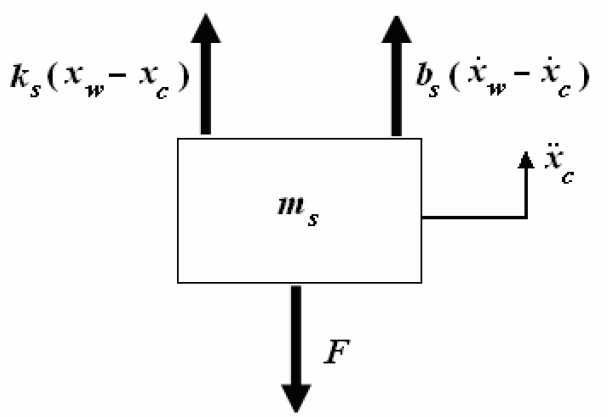
\includegraphics[width=8cm,height=6cm]{img/corpo_livre_ms.png}
            \caption{Diagrama de corpo livre para a massa $m_s$.} 
            \label{fig:corpo_livre_ms}
        \end{centering}
\end{figure}
\FloatBarrier
\begin{figure}[htbp]
    \begin{centering}
        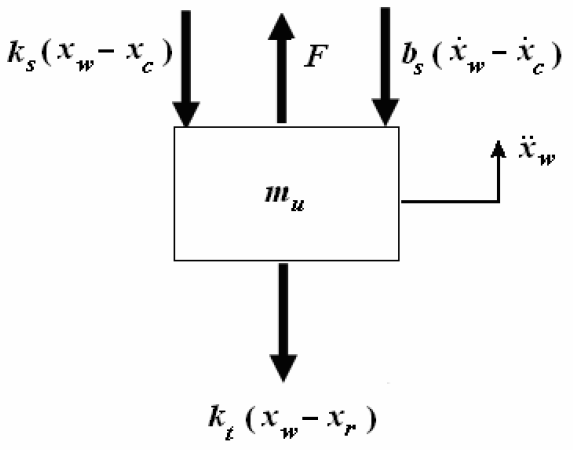
\includegraphics[width=8cm,height=6cm]{img/corpo_livre_mu.png}
        \caption{Diagrama de corpo livre para a massa $m_u$.} 
        \label{fig:corpo_livre_mu}
    \end{centering}
\end{figure}
\FloatBarrier
    
Aplicando a segunda lei de Newton $\sum{F}=m.a$, a cada uma das massas separadamente, o sistema para o modelo de um quarto de carro da figura \ref{fig:massa_mola_nao_linear_controlavel} pode ser representado pela seguinte equação:
    
\begin{equation} \label{eq:massa_mola_linear}
    \begin{split}
        m_{s} \ddot{x}_{c} =&  b_{s}(\dot{x}_{w}-\dot{x}_{c}) + k_{s}(x_{w}-x_{c}) - F\ \\
        m_{u} \ddot{x}_{w} =& -b_{s}(\dot{x}_{w}-\dot{x}_{c}) - k_{s}(x_{w}-x_{c})+k_{t}(x_{w}-x_{r}) + F
    \end{split}
\end{equation}
    
A equação \ref{eq:massa_mola_linear} representa o modelo do sistema na forma linear. Porém a mola $k_s$, o amortecedor $b_s$ e o amortecedor dinâmico ativo podem ser modelados através de modelos lineares ou modelos não lineares. \\
Uma mola linear obedece a lei de Hooke apresentando uma deformação proporcional ao carregamento. Em uma mola não linear o coeficiente de elasticidade da mola cresce exponencialmente conforme se afasta do ponto de equilíbrio estático.
Para um modelo de mola não linear, podemos utilizar seguinte expressão para a força da mola $ k_{s}(x_{w}-x_{c})$:
    
\begin{equation} \label{eq:mola_nao_linear}
    k_{s}(x_{w}-x_{c}) = k^{l}_{s}(x_{w}-x_{c})+k^{nl}_{s}(x_{w}-x_{c})^{3}
\end{equation}
        
Na equação \ref{eq:mola_nao_linear} o coeficiente $k^{l}_{s}$ representa o coeficiente de elasticidade do termo da faixa de operação linear e o coeficiente $k^{nl}_{s}$] representa o coeficiente de elasticidade do termo da faixa de operação não linear do feixe de molas em uma situação real.\\
A não linearidade do amortecedor permite que pequenos movimentos causados pelo perfil da estrada gerem apenas um pequeno impacto na carroceria além de apresentar saturação e histerese. Para um modelo de amortecedor não linear, podemos utilizar a seguinte expressão:
 
\begin{equation} \label{eq:amortecedor_nao_linear}
    \begin{aligned}
        b_{s}(\dot{x}_{w}-\dot{x}_{c}) =\ \ &b^{l}_{s}(\dot{x}_{w}-\dot{x}_{c}) - b^{y}_{s}\mid\dot{x}_{w}-\dot{x}_{c}\mid \\
        + &b^{nl}_{s}\sqrt{\mid\dot{x}_{w}-\dot{x}_{c}\mid}sgn(\dot{x}_{w}-\dot{x}_{c})  
    \end{aligned}
\end{equation}
    
Na equação \ref{eq:amortecedor_nao_linear} o coeficiente $b^{l}_{s}$ representa o coeficiente de amortecimento do termo da faixa de operação linear, o coeficiente $b^{l}_{s}$ representa o coeficiente de amortecimento do termo da faixa de operação não linear e o coeficiente $b^{y}_{s}$ representa a característica de comportamento assimétrico do amortecedor.
    
Substituindo as equações \ref{eq:mola_nao_linear} e \ref{eq:amortecedor_nao_linear} em \ref{eq:massa_mola_linear}, obtemos as seguintes equações diferenciais dinâmicas de segunda ordem que, representam a dinâmica de um sistema de suspensão ativa não linear:
    
\begin{equation} \label{eq:massa_mola_nao_linear}
    \begin{aligned}
         m_{s} \ddot{x}_{c} =\ \ &k^{l}_{s}(x_{w}-x_{c})+k^{nl}_{s}(x_{w}-x_{c})^{3}+b^{l}_{s}(\dot{x}_{w}-\dot{x}_{c})\\
                            -&b^{y}_{s}\mid\dot{x}_{w}-\dot{x}_{c}\mid+b^{nl}_{s}\sqrt{\mid\dot{x}_{w}-\dot{x}_{c}\mid}sgn(\dot{x}_{w}-\dot{x}_{c})\\ 
                            -&F\\
         m_{u} \ddot{x}_{w} = -&k^{l}_{s}(x_{w}-x_{c})-k^{nl}_{s}(x_{w}-x_{c})^{3}-b^{l}_{s}(\dot{x}_{w}-\dot{x}_{c})\\  
                            +&b^{y}_{s}\mid\dot{x}_{w}-\dot{x}_{c}\mid-b^{nl}_{s}\sqrt{\mid\dot{x}_{w}-\dot{x}_{c}\mid}sgn(\dot{x}_{w}-\dot{x}_{c})\\
                            -&k_{t}(x_{w}-x_{r})+F\\
    \end{aligned}
\end{equation}
        
\subsection{Modelo Linearizado de um sistema de suspensão semi-ativa, não linear, de um quarto de veículo, com dois graus de liberdade }
Realizando a distributiva no sistema descrito em \ref{eq:massa_mola_nao_linear} e propondo as seguintes substituições para as variáveis de estado das equações e reorganizando os termos, obtemos: 
\begin{equation*}
    \begin{split}
        x_{1}=&x_{c};\ \ \\
        x_{2}=&\dot{x}_{c};\ \ \\ 
        x_{3}=&x_{w};\ \ \\               
        x_{4}=&\dot{x}_{w};\ \ \\
    \end{split}
    \begin{split}
        \dot{x}_{1}=&\dot{x}_{c};\ \ \\
        \dot{x}_{2}=&\ddot{x}_{c};\ \ \\
        \dot{x}_{3}=&\dot{x}_{w};\ \ \\        
        \dot{x}_{4}=&\ddot{x}_{w};\ \ \\
    \end{split}
    \begin{split}
        w=&x_{r};\ \ \\
        u=&F;\ \ \\
    \end{split} 
\end{equation*}
\begin{equation} \label{eq:massa_mola_nao_linear_SS}
    \begin{aligned}
        \dot{x}_{1}=&\ \ \ \ x_{2}\\        
        \dot{x}_{2}=&-\frac{k^l_s}{m_s}x_1-\frac{b^l_s}{m_s}x_2+\frac{k^l_s}{m_s}x_3+\frac{b^l_s}{m_s}x_4-\frac{k^{nl}_s}{m_s}(x_3-x_1)^3\\
                    &+\frac{b^y_s}{m_s}\mid x_4-x_2\mid+\frac{b^{nl}_s}{m_s}\sqrt{\mid x_4-x_2\mid}sgn(x_4-x_2)\\
                    &-\frac{1}{m_s}u\\    
        \dot{x}_{3}=&\ \ \ \ x_{4}\\
        \dot{x}_{4}=&\ \ \ \ \frac{k^l_s}{m_u}x_1+\frac{b^l_s}{m_u}x_2-\frac{k^l_s}{m_u}x_3-\frac{b^l_s}{m_u}x_4+\frac{k^{nl}_s}{m_u}(x_3-x_1)^3\\
                    &-\frac{b^y_s}{m_u}\mid x_4-x_2\mid-\frac{b^{nl}_s}{m_u}\sqrt{\mid x_4-x_2\mid}sgn(x_4-x_2)\\
                    &+\frac{k_t}{m_u}w+\frac{1}{m_u}u\\
    \end{aligned}
\end{equation}
    
\subsection{Linearização de um modelo em espaço de estados}
Um sistema dinâmico descrito por meio de equações diferenciais não lineares, pode ser linearizado na proximidade de um ponto de equilíbrio, através do método da expansão em série de Taylor truncada no seu segundo termo como exibido na equação a seguir:
    
\begin{equation}
        P(x) = f(\alpha) + \dfrac{\mathrm{d}f(\alpha)}{\mathrm{d}x}*\frac{(x-\alpha)^{-1}}{1!}    
\end{equation}
    
Onde $\alpha$ é um ponto de equilíbrio da equação $P(x)$.  
Para um sistema com múltiplas variáveis de estado, calcula-se a Jacobiana do sistema para realizar a linearização em torno do ponto de operação escolhido.  
    
\begin{equation} \label{eq:Jacobian_A}
    \mathbf{J_A}(x_1,x_2,\dots,x_n) =
    \begin{bmatrix}
        \frac{\partial x_1}{\partial x_1} & 
        \frac{\partial x_1}{\partial x_2} & 
        \dots &
        \frac{\partial x_1}{\partial x_n} &\\[1ex]
        \frac{\partial x_2}{\partial x_1} & 
        \frac{\partial x_2}{\partial x_2} & 
        \dots &
        \frac{\partial x_2}{\partial x_n} &\\[1ex]
        \vdots & 
        \vdots & 
        \ddots &
        \vdots &\\[1ex]
        \frac{\partial x_n}{\partial x_1} & 
        \frac{\partial x_n}{\partial x_2} & 
        \dots &
        \frac{\partial x_n}{\partial x_n} &\\[1ex]
    \end{bmatrix}
\end{equation}
    
    \begin{equation} \label{eq:eval_A}
        \mathbf{A=J_A} \Bigr\rvert_{(x_1=\alpha_1;x_2=\alpha_2;\dots;x_n=\alpha_n)} \\
    \end{equation}
    
    \begin{equation} \label{eq:Jacobian_B}
    \mathbf{J_B}(u_1,u_2,\dots,u_m) =
        \begin{bmatrix}
            \frac{\partial u_1}{\partial u_1} & 
            \frac{\partial u_1}{\partial u_2} & 
            \dots &
            \frac{\partial u_1}{\partial u_m} &\\[1ex]
            \frac{\partial u_2}{\partial u_1} & 
            \frac{\partial u_2}{\partial u_2} & 
            \dots &
            \frac{\partial u_2}{\partial u_m} &\\[1ex]
            \vdots & 
            \vdots & 
            \ddots &
            \vdots &\\[1ex]
            \frac{\partial u_n}{\partial u_1} & 
            \frac{\partial u_n}{\partial u_2} & 
            \dots &
            \frac{\partial u_m}{\partial u_m} &\\[1ex]
    \end{bmatrix}
    \end{equation}
    
    \begin{equation} \label{eq:eval_B}
        \mathbf{B=J_B} \Bigr\rvert_{(u_1=\beta_1;u_2=\beta_2;\dots;u_m=\beta_m)} \\
    \end{equation}
    
    \begin{equation} \label{eq:sis_lenearizado}
        Y(x,u) = A*x + B*u
    \end{equation}
    
     Onde:
     \begin{itemize}
        \item $x=[x_1,x_2,\dots,x_n]$ o vetor de estados do sistema
        \item $u=[u_1,u_2,\dots,u_m]$ o vetor das entradas do sistema
        \item $\alpha=[\alpha_1,\alpha_2,\dots,\alpha_n]$ um vetor solução para os pontos de equilíbrio dos estados do sistema.
        \item $\beta=[\beta_1,\beta_2,\dots,\beta_m]$ um vetor solução para os pontos de equilíbrio das entradas do sistema.
        \item $Y(x,u)$ equação do sistema linearizado ao redor do ponto de equilíbrio $\alpha$.
     \end{itemize}
     
    
\subsection{Especificações da Resposta Transitória para Sistemas Subamortecidos}
As características de um sistema de controle são geralmente especificadas em termos da resposta transitória para uma entrada em degrau. Para sistemas LIT, quando a resposta ao degrau é conhecida, pode-se calcular a resposta a qualquer tipo de entrada e costuma-se utilizar condição inicial de sistema em repouso. As seguintes especificações são as mais utilizadas:
\begin{itemize}
    \item  Tempo de atraso - $t_d$: tempo necessário para que a resposta alcance metade do seu valor final pela primeira vez.
    \item  Tempo de subida - $t_r$: tempo requerido para que a resposta passe de 10\% a 90\%, ou de 5\% a 95\%, ou de 0\% a 100\% do valor final. Para sistemas de 2ª ordem subamortecido, utiliza-se 0\% a 100\% do valor final. Para sistemas superamortecidos, geralmente considera-se de 10\% a 90\%.
    \begin{equation} \label{eq:tr}
        t_r = \frac{\pi-\theta}{\omega_d}
    \end{equation} 
    \item Tempo de pico - $t_p$: tempo para que a resposta atinja o primeiro pico de sobressinal.
    \begin{equation} \label{eq:tp}
        t_p = \frac{\pi}{\omega_d}
    \end{equation}
    \item Máximo overshoot $MO$: valor máximo de pico da curva de resposta, medido a partir da unidade. Se o valor da resposta em regime diferir da unidade, utiliza-se a porcentagem máxima de sobressinal (ou ultrapassagem percentual, U.P.):
    \begin{equation} \label{eq:MaxOv}
        \begin{split}
            M_O=\exp{(\frac{-\xi.\pi}{\sqrt(1-\xi^2)})}\\
            \xi=-\frac{ln\left( M_O \right)}{\sqrt{\pi^2+ln^2(M_O)}}
        \end{split}
    \end{equation}
    \item Tempo de acomodação ou assentamento - $t_s$: tempo necessário para que a resposta permaneça com valores no interior de uma certa faixa (usualmente $\pm2\%$ ou $\pm5\%$) em torno do valor final.
    \begin{equation} \label{eq:Ts2}
        \begin{split}
            T_{S_{2\%}}=-\frac{ln\left( 0.02*\sqrt{1-\xi} \right)}{\omega_n*\xi}\\
            \omega_n=-\frac{ln\left( 0.02*\sqrt{1-\xi} \right)}{T_{S_{2\%}}*\xi}  
        \end{split}
    \end{equation}
\end{itemize}

Dado que:
\begin{equation} \label{eq:eign}
        \lambda = \sigma \pm \omega_d.i
\end{equation}
\begin{equation} \label{eq:xi}
    \xi=\frac{\sigma}{|\omega_n|}
\end{equation}
\begin{equation} \label{eq:theta}
        \xi=\cos{(\theta)}
\end{equation}
\begin{equation} \label{eq:wd}
        \omega_d=\omega_n\sqrt{1-\xi^2}
\end{equation}
    
\subsection{Observador de Luenberger}\label{sc:luemberger}

Considere o sistema linear e invariante no tempo representado a seguir pela equação \ref{eq:linsys}:

\begin{equation}\label{eq:linsys}
    \begin{split}
        \dot{x}(t)=&Ax(t)+B_uu(t)+B_ww(t)\\
              y(t)=&Cx(t)+D_uu(t)+D_ww(t)
    \end{split}
\end{equation}

Considere também o observador de estados linear de Luenberger representado a seguir pela equação \ref{eq:linLue}: 

\begin{equation}\label{eq:linLue}
    \begin{split}
        \hat{\dot{x}}(t)=&(A-LC)\hat{x}(t) + Ly(t) 
    \end{split}
\end{equation}

Onde $x \in \Re^{n*1}$ é o vetor de estados do sistema, $u \in \Re^{r*1}$ é o vetor de entrada de controle, $w \in \Re^{p*1}$ é o vetor de entrada de perturbação, $A \in \Re^{n*n}$, $B \in \Re^{n*1}$, $C \in \Re^{m*n}$, $D_u \in \Re^{1*1}$ e $D_w \in \Re^{1*1}$ são as matrizes do sistema, $y \in \Re^{m*1}$ é o vetor de saídas, $z \in \Re^{n*1}$ é o vetor de estados preditos, e $L\in \Re^{n*1}$ é o vetor de ganhos do observador.

Considere o par $(A,C)$ completamente observável. O que implica que a matriz de observabilidade:

\begin{equation}\label{eq:Matrix:MO}
    \mathbb{M_O}=
    \begin{bmatrix}
        C^'&A^'C^'&(A^')^2C^'&\dots&(A^')^{n-1}C^'\\
    \end{bmatrix}        
\end{equation}

Possui $rank(\mathbb{M_O}) = n$
 
Se o par $(A,C)$ for completamente observável é possível encontrar um vetor de ganhos $L\in \Re^{n*1}$ que faça com que o conjunto de autovalores de $A-L*C$ corresponda ao conjunto de autovalores de qualquer matriz $F \in \Re^{n*n}$ arbitrariamente escolhida. 
Definindo-se o erro de estimação de estado como $e=x-\hat(x)$, $L$ deve ser escolhido de maneira que leve $(A-LC)$ à estabilidade rapidamente e sem grandes oscilações), ou seja, L deve fazer com que o erro de observação e,
qualquer que seja o erro inicial, convirja para zero o mais rapidamente possível. Para isso, é muito importante que o observador seja mais rápido 
que o sistema que ele observa, assim ele não introduz erros significativos na dinâmica do sistema controlado. A escolha conveniente dos autovalores de $(A-LC)$ faz com que o erro $e\rightarrow0$ assintoticamente. 
O conjunto de autovalores de $(A-LC)$ pode ser escolhida pela resolução da equação de Lyapunov.
    
\begin{enumerate}
    \item Define-se uma matriz $F \in \Re^{n*n}$ com os autovalores desejados, pelo menos 3 vezes mais rápidos do que o autovalor mais rápido do sistema.
    \item Escolhe-se uma matriz $\bar{k}$ arbitrário tal que $(F,\bar{k})$ seja observável.
    \item {Obtém-se a solução única $T$ da equação de Lyapunov
    \begin{equation} \label{eq:lyapunov}
            A'T-TF=C'\bar{k}
    \end{equation}}
    \item {Computa-se o ganho de realimentação:
    \begin{equation} \label{eq:ganho}
            L=\bar{k}T^{-1}
    \end{equation}}
\end{enumerate}  

A implementação do observador de Luenberger em ambiente Simulink é exibida na figura \ref{fig:luemberger_simulink} a seguir:

\FloatBarrier
\begin{figure}[htbp]
    \begin{centering}
        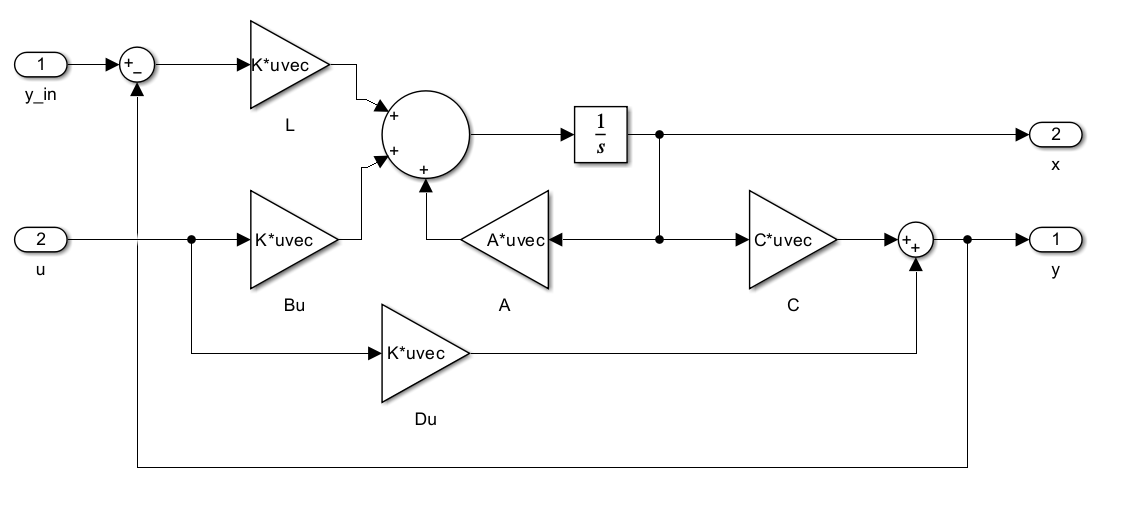
\includegraphics[width=8cm]{img/luenberger_simulink.png}
        \caption{Observador de Luenberger em ambiente Simulink.} 
        \label{fig:luemberger_simulink}
    \end{centering}
\end{figure}
\FloatBarrier